%%%%%%%% Chapters %%%%%%%%%%%%
%% Introduction
\newcommand\tab[1][1cm]{\hspace*{#1}}
\chapter{Introduction and Background}
\label{chap:introduction}

\section{AmericasNLP Shared Task}
The AmericasNLP 2024 Shared Task \cite{americasnlp2024} focuses on the development of   machine translation (MT) systems for Indigenous languages of the Americas. Specifically, the competition encourages participants to build MT systems that translate from Spanish into 11 different Indigenous languages. This task aims to address the unique challenges posed by low-resource languages, which often lack sufficient parallel data to train effective translation models. Additionally, many Indigenous languages feature linguistic properties that are less common in the more frequently studied languages. By organizing this shared task, AmericasNLP seeks to motivate researchers to tackle these challenges and improve the accessibility of machine translation for Indigenous language speakers.
Those participating in the shared task are invited to use provided training and development data, but are also free to incorporate additional resources, including pretrained models, as strategy that has been successful in the past. The primary evaluation metric for the competition is ChrF++, a character n-gram-based metric for assessing the quality of machine translations. With the goal of improving MT quality and digital representation of indigenous diversity,  the competition's evaluation process will assess individual language pairs as well as an overall average score to determine the winner. In this task, the translation direction is always from Spanish to the indigenous language. Specifically the language pairs with data provided and evaluated are: 
\begin{itemize}
    \item Hñähñu–Spanish
    \item Wixarika–Spanish
    \item Nahuatl–Spanish
    \item Guaraní–Spanish
    \item Bribri–Spanish
    \item Rarámuri–Spanish
    \item Quechua–Spanish
    \item Aymara–Spanish
    \item Shipibo-Konibo–Spanish
    \item Asháninka–Spanish
    \item Chatino–Spanish    
\end{itemize}


\section{The Transformer Architecture}
The introduction of the Transformer architecture in "Attention Is All You Need" \cite{NIPS2017_3f5ee243} marked a paradigm shift in machine translation (MT) and natural language processing more broadly. To understand its significance, consider the fundamental challenge in machine translation: capturing the relationships between words in diverse languages while preserving meaning and structure. Previous approaches relied heavily on recurrent neural networks (RNNs) and long short-term memory (LSTM) networks. These models use recurrence and convolution and therefore processing text sequentially—word by word—much like a human reader. While effective, these sequential models struggled with long-range dependencies due to the positive linear relationship of distance between tokens and number of computations needed to relate them. This made accounting for long-range dependencies between tokens both costly and ineffective in RNN and LTSM networks. 

Take this example sentence, “The keys to the car are there” where the subject “keys” and the verb “are” are linked despite their relatively large distance in the sentence. This example of subject-verb resolution highlights why understanding long-range dependencies in sentences is important.  Additionally, due to the sequential nature of this evaluation, these models were inherently limited in their ability to parallelize computation and therefore were costly both temporally and spatially. 

To ground our discussion, let's consider a simple Spanish sentence that will serve as our running example throughout this section: "El gato negro duerme en la casa" (The black cat sleeps in the house). This sentence, while straightforward, encompasses several key challenges in machine translation, including word order differences, agreement, and contextual relationships.

\subsection{A High-Level View of the Transformer}

The Transformer's revolutionary approach lies in its complete abandonment of recurrence in favor of attention mechanisms. Instead of processing words sequentially, the Transformer considers all words in a sentence simultaneously, weighing their relationships to each other directly. This parallel processing capability not only accelerates training but also allows the model to capture complex relationships between words regardless of their distance in the sentence.

A transformer is made up of blocks, and as an input travels through the transformer blocks, the initial inputs become contextual embeddings. As these contextual embeddings pass through more layers, they gain richer and richer meaning. In machine learning models, meaning is gained through context, so the more context an embedding is able to account for, the more meaningful it is. In the early layers of the transformer the model gains an understanding of syntax and position while later layers embed the semantics of the sequence. 

In our example sentence, traditional sequential models would need to process each word in order. Therefore, they potentially would struggling to maintain the relationship between "gato" and "negro" when generating translations where adjective placement differs. For example, in English we would say “black cat” which switches the word order of “gato” and “negro.” The Transformer, in contrast, can immediately establish these relationships through its attention mechanism.

\subsection{The Building Blocks of Transformer Architecture}

\subsubsection{Attention Mechanisms in the Transformer}
The core innovation of the Transformer is the attention mechanism, which enables it to focus on different parts of the input sequence with varying intensity, or "attention." In the Transformer, this mechanism is implemented as scaled dot-product attention, which computes the relevance of each word in the sequence relative to others using query, key, and value vectors. Here’s how this works in more detail:

\subsubsection{Self-Attention}
In the self-attention mechanism, each word (or token) in a sequence is represented as a query, a key, and a value. These vectors are created by projecting the original embedding of each word through learned weight matrices: \\
\tab[1cm]$Q =WQX, K =WKX, V = WVX $ \\
where $Q$, $K$ , and $V$ are the query, key, and value matrices, respectively, and $X$ is the input matrix of embeddings. The attention score between two tokens is calculated by taking the dot product of the query vector for one token and the key vector of another, scaled by the square root of the dimension ($d_k$) to stabilize gradients:\\
\tab[1cm]$Attention(Q, K, V) = softmax(\frac{QK^T}{\sqrt{d_k}})V$ \\
This operation generates a weight for each relevant token pair, enabling the model to weigh the importance of each word to another. After obtaining these attention weights, the model calculates a weighted sum of the values to create the output representation.

\subsubsection{Masked Self-Attention}
For the decoder stack, the Transformer incorporates a variant called masked self-attention. This is crucial for generating sequences (like translations) where each word prediction depends only on the words generated so far. Masked self-attention prevents the model from attending to “future” tokens by applying a mask over the attention weights, effectively blocking connections from later positions to earlier ones. With the mask the equation becomes: \\
	\tab[1cm]$Attention(Q, K, V) = softmax(mask(\frac{QK^T}{\sqrt{d_k}}))V$ \\
In practice, the mask is a matrix where the — triangle of the matrix is $-\infty$. When multiplied this effectively zeros out all tokens that come sequentially after token i in the sequence. Here is an example of a mask matrix for a small, toy example.This, when applied, would zero out all of the elements at the positions with the negative infinity values, ensuring that the prediction can only come from past information, mimicking next token prediction. Here is an example of a masking matrix: 
    \[
\begin{bmatrix}
    1 & -\infty & -\infty \\
    1 & 1 & -\infty \\
    1 & 1 & 1
\end{bmatrix}
\]

\subsubsection{Multi-Head Attention}
A single attention head captures one aspect of the relationships in the sequence. To capture richer, more diverse relationships, the Transformer employs multiple attention heads, each with its own set of query, key, and value matrices:\\
	\tab$MultiHead(Q, K, V) = Concat(head_1,\dots,head_h)WO $ \\
	\tab Where each $head_i =Attention(QW_iQ,KW_iK, VW_iV) $ \\
where each head performs the attention operation in parallel. In this model, there are 8 attention heads working in parallel. These outputs are concatenated and projected through a final weight matrix ($WO$). This design allows each head to focus on different aspects of language, such as syntactic or semantic relationships, and combine them to form a more comprehensive representation of the input.

\subsubsection{Layer Norm}
Layer normalization is a technique used in the Transformer architecture to help stabilize the training process. It normalizes the inputs to a layer by subtracting the mean and dividing by the standard deviation of the layer's activations, helping to reduce internal output shift.

\subsubsection{Position-Wise Feed Forward Network}
After the multi-head self-attention, each token undergoes processing through a fully connected feed-forward network, which is applied independently to each position in the sequence. The network consists of two linear transformations with a ReLU activation in between. The input and output dimensions are both 512, while the inner layer has 2048 units.

\subsection{Full Architecture and a Journey Through a Transformer}

\subsubsection{Input Processing}
The journey of our example sentence through the Transformer begins with tokenization and embedding. Each word is converted into a dense vector representation, but unlike previous models, the Transformer must explicitly encode position information since it lacks the implicit ordering of sequential models. This is accomplished through positional encodings—sinusoidal functions that give each token a unique position signature. \\

Input: "El gato negro duerme en la casa" \\ 

Tokens: ["El", "gato", "negro", "duerme", "en", "la", "casa"] \\

Each token is embedded into a 512-dimensional vector (in the base model), and positional encodings are added to maintain sequence information.

\subsubsection{The Encoder Stack}
The encoder consists of six identical layers, each containing two sub-layers: a multi-head self-attention mechanism and a position-wise dense feed-forward network. The self-attention mechanism allows each word to attend to all other words in the sentence up to and including itself, capturing contextual relationships. In our example, when processing "negro," the attention mechanism might focus heavily on "gato" to establish agreement, while also maintaining awareness of other contextual elements. 

The multi-head attention mechanism can be visualized as multiple parallel attention computations, each potentially focusing on different aspects of the relationships between words. For instance, one attention head might focus on grammatical structure, while another captures semantic relationships. Each sub-layer in the encoder layer is wrapped with residual connections, followed by layer normalization, which helps stabilize the training process. The combination of multi-head self-attention and feed-forward layers allows the encoder to produce a rich, contextualized representation of the input sequence. 

Therefore, the output of each sublayer is: \\
	\tab$LayerNorm(x + Sublayer(x))$ for each sublayer in a transformer block. \\
For encoders, we see that the two sublayers are a FFN which is then fed into and a multi-attention head. For the decoder stack, the logic is the same but with one additional sublayer. 

In our example, the tokenized and embedded Spanish inputs are passed into the encoder, which consists of six identical transformer blocks. Within each block, the self-attention mechanism allows each word to dynamically attend to all other words in the sequence, capturing important contextual relationships.

For example, when processing the token "negro" (black), the self-attention mechanism might focus heavily on "gato" (cat) to establish the correct grammatical agreement, while also maintaining awareness of other relevant context like "duerme" (sleeps) and "en" (in). The multi-head design of the attention mechanism enables it to capture diverse linguistic phenomena, such as syntactic and semantic connections. After the self-attention sub-layer, the position-wise feed-forward network further refines the contextual representations of each token. This combination of attention and feed-forward processing allows the encoder to produce rich, contextualized embeddings for the entire input sequence.

\begin{figure}[h!]
    \centering
    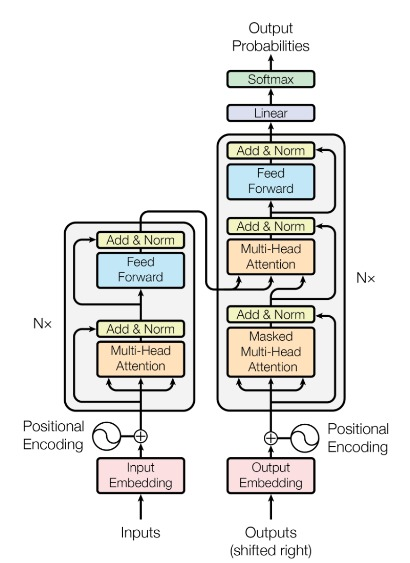
\includegraphics[width=0.5\textwidth]{chapters/transformer.jpeg} 
    \caption {The Diagram shows the transformer architecture. \cite{NIPS2017_3f5ee243} On the left is a single encoder block and on the right is a single decoder block. In use, multiple of each of these blocks would be stacked on themselves, and the outputs from the final encoder block would be added at the multi-head attention stage of each decoder block.}
\end{figure}

\subsubsection{The Decoder Stack}
The decoder, crucial for our translation task, also contains six layers but with an additional sub-layer for attending to the encoder's output. This extra sublayer, the masked-multi attention head comes before the other two layers, is subject to the same residual addition and layer norming. Because of this new sublayer, the decoder's operation is particularly interesting as it must generate text auto-regressively (one word at a time taking into account the previous words it has predicted) despite the parallel nature of the architecture. Here, the input to the decoder is the the output of the encoder and the previous outputs of decoder block itself. 

Consider the generation process for our example sentence: \\
\begin{enumerate}
    \item The decoder starts with a special "begin" token and predicts for the next position
    \item Each generated word attends to:
    \begin{itemize}
        \item Previously generated words (through masked self-attention)
        \item The entire encoded source sentence (through encoder-decoder attention)
    \end{itemize}
        \item The decoder block generates a predicted next token for the given position
    \begin{itemize}
        \item This prediction is given back to the start of the decoder block as input
        \item The model autoregressive predicts the next token, returning to step 2 
    \end{itemize}
    \item The process continues until a special "end" token is generated
\end{enumerate}

The masked self-attention in the decoder ensures that predictions for each position can depend only on known outputs at previous positions—a crucial feature for maintaining coherent translations. The encoder-decoder attention links the final contextual embeddings of the whole encoder stack to be added as input into the second sublayer, the multi-attention head. 

Using our running example, we can see how the decoder, a crucial step for generating the translated output, generates the translation. Let's consider the decoding process step-by-step: \\
\begin{enumerate}
    \item The decoder starts with a special start token and predicts the first output word. 
    \item For each subsequent position, the decoder's masked self-attention sub-layer only attends to the previously generated tokens, ensuring that predictions depend only on the known output so far.
    \begin{itemize}
        \item For example, When predicting the for position 3 which is suppose to be "duerme", the decoder model will autoregressivly look at the predicted tokens for ["el", "gato", "negro"]. 
    \end{itemize}
    \item For example, if predicting position 1, the model could use this context found by scaled dot product attention and weights tuned to spanish-english translation to know to predict “black” for position two even though the second position of the input was “gato”.
    \begin{itemize}
        \item For example, When predicting the for position 3 which is suppose to be "duerme", the decoder model will autoregressivly look at the predicted tokens for ["el", "gato", "negro"]. 
    \end{itemize}
    \item Finally, the position-wise feed-forward network processes the attended encoder and decoder representations to produce the prediction for the current output position.
    \item The predicted token is then fed back into the decoder block, and the process repeats until a special "end" token is generated, signaling the completion of the translation.
\end{enumerate}

This autoregressive, step-by-step decoding process, combined with the masked self-attention, allows the Transformer to maintain coherence and fluency in the generated translations, despite its inherently parallel architecture. By seamlessly integrating the encoder's contextual understanding of the input with the decoder's step-by-step generation of the output, the Transformer is able to capture the complex relationships between words in diverse languages, enabling high-quality machine translation.

\subsection{Advantages and Implications for Low-Resource Languages}
The Transformer's architecture offers several advantages particularly relevant to low-resource language translation:
\begin{itemize}
    \item Efficient parameter sharing through attention mechanisms
    \item Strong ability to capture long-range dependencies
    \item Potential for transfer learning from high-resource to low-resource languages
\end{itemize}

The parallel processing capability significantly reduces training time compared to sequential models, while the attention mechanism's ability to capture long-range dependencies is particularly valuable for languages with different word order patterns.

Understanding the Transformer architecture is crucial for modern MT work, as it forms the foundation for current state-of-the-art models, the previous best models for the AmericasNLP competitions, and continues to influence new architectural innovations in the field. Its ability to handle complex linguistic relationships while maintaining computational efficiency makes it particularly suitable for multilingual and low-resource translation tasks.

\section{No Language Left Behind}
The research paper "No Language Left Behind: Scaling Human-Centered Machine Translation" \cite{nllbteam2022languageleftbehindscaling} presents an innovative approach to expanding machine translation (MT) technology to include over 200 languages, with a focus on low-resource languages that have been historically underrepresented and difficult to translate. These languages, often spoken by smaller communities, have had limited access to machine translation services, thus exacerbating communication and information gaps. The authors aimed to develop a system that delivers high-quality, safe translations while addressing the needs and values of the communities using these languages. 

In order to align the machine translation technology with the needs of speakers of low-resource languages, the authors conducted interviews with individuals from these communities. The goal was to gather qualitative insights into their expectations and concerns regarding machine translation. These interviews revealed a number of key themes that informed the guiding principles of the project. First, participants expressed high expectations for improved communication and better access to knowledge resources, such as Wikipedia, which they saw as essential for educational advancement. Second, while many were aware of existing translation systems for their languages, concerns about translation quality and limitations in script and dialect support were frequently raised. Finally, there was a strong desire for greater representation and visibility, with respondents noting that inclusion in commercially available translation services would be a significant step toward increasing the global recognition of their languages.

The researchers identified four guiding principles for the NLLB (No Language Left Behind) project based on the interview insights and responsible AI frameworks. These principles are prioritizing the needs of underserved communities, ensuring that the historical imbalance in digital representation is addressed, ensuring high-quality translations that are both grammatically correct and contextually appropriate for real-world applications, mitigating potential harms associated with machine translation, such as the generation of biased or harmful content, and promoting open-source datasets and models to encourage broader adoption and further research in low-resource language translation.
To achieve these goals, the NLLB project focuses on expanding language coverage and creating high-quality datasets to train its models. The authors highlight the creation of several key datasets that form the backbone of the NLLB project. The FLORES-200 dataset, a benchmark translation resource covering 204 languages, is central to the project's multilingual approach. Additionally, the NLLB-Seed dataset was developed for 39 low-resource languages, offering vital translation data in cases where publicly available data was scarce. These datasets are instrumental in overcoming the challenges of data scarcity and improving the performance of machine translation models for low-resource languages.

The NLLB team also explored several modeling innovations that enhance the translation quality for low-resource languages, particularly in the face of limited training data. One key advancement is the use of conditional computation through Sparsely Gated Mixture-of-Experts (MoE) models. These models activate specialized expert subnetworks for different parts of the input data by training a gating system to activate one of many FFN experts in a transformer block, optimizing model capacity and improving translation accuracy. The authors also introduced techniques such as Expert-Oriented Model Selection (EOM), which prioritizes model checkpoints based on performance in low-resource languages, and curriculum learning, which presents training data in a progressive manner to facilitate more effective learning from limited data.

Additional techniques such as backtranslation, datafiltering, and the use of self-supervision strategies further strengthen the NLLB model’s capabilities. Backtranslation generates additional training data by translating target language data back into the source language, improving fluency and accuracy. Rigorous data filtering ensures that the training data is of high quality, removing sentence pairs that are poorly aligned, excessively long or short, or contain toxic language.

The NLLB project represents a significant step forward in making machine translation accessible and effective for low-resource languages. By combining a human-centered approach with innovative modeling techniques and comprehensive datasets, the project aims to bridge communication gaps and increase the visibility and utility of low-resource languages on a global scale. The guiding principles and modeling innovations outlined in the paper reflect a commitment to not only improving the technical performance of machine translation systems but also ensuring that they are ethically sound and inclusive of linguistic communities.

\section{University of Sheffield Submission}
In the 2023 AmericasNLP Shared Task, the University of Sheffield successfully tackled Shared Task 1, making large improvements in the translations of many of the language pairs \cite{gow-smith-snchez-villegas-2023-sheffields}. During their research development, the University of Sheffield team stressed that the language pairs presented significant translation difficulties due to their polysynthetic structures, unstandardized word boundaries, and limited available training data. The research team adopted a comprehensive approach to addressing these challenges, drawing inspiration from recent advances in machine translation technology. The University of Sheffield's research team approached this challenge by fine-tuning the NLLB-200 (No Language Left Behind). Their methodology involved an extensive data collection strategy that went far beyond the initial training data provided by the task organizers. The team compiled parallel texts from diverse sources, including constitutional documents, news articles, literary works, and even Bible translations, ultimately creating a comprehensive dataset for each target language.

To prepare the data, the researchers conducted detailed preprocesses, addressing challenges such as tokenization inconsistencies and vocabulary limitations. In particular, they changed the tonal super scripts of Chatino into standard, capital letters, and detokenzied the already tokenized data for the Nahuatl and Hñähñu bitexts supplied by AmericasNLP. Additionally, they found that 7\% of the characters in the Hñähñu dataset were outside of the NLLB tokenizer vocabulary, but they did not address this issue. They experimented with multiple versions of the NLLB-200 model, ranging from 600 million to 3.3 billion parameters, and implemented a multilingual training approach that allowed knowledge transfer across the different indigenous languages.

Their data collection was comprehensive, drawing from multiple sources including the AmericasNLP 2023 dataset, Helsinki University's corpus, REPUcs submissions, NLLB datasets, and Bible translations. The total training data varied dramatically across languages, with Quechua having the most substantial corpus at 557,277 examples, while Chatino had merely 3,118 parallel examples. Backtranslation, a technique of generating additional training data by translating target language text back to the source language, was also conducted but proved selective in its effectiveness. The team generated backtranslations for seven languages using monolingual data, but found performance improvements only for Guarani and Shipibo-Konibo. This selective success highlighted the importance of having sufficient monolingual data for this technique to be effective.

The researchers primarily utilized the NLLB-200 model, experimenting with different parameter sizes: 600 million, 1.3 billion, and 3.3 billion. While the 3.3B model showed superior performance in initial inference tests, computational constraints led them to conduct most experiments with the 1.3 billion parameter version. Their final submission, Submission 3, used a single best NLLB-1.3B model trained multilingually, choosing the checkpoint with the highest average chrF score. Multilingual training emerged as a crucial strategy. They hypothesized that by training the model simultaneously on all eleven language pairs, enabled knowledge transfer across languages. This approach was particularly beneficial for Quechua, where a model trained only on Quechua data performed significantly worse than the multilingual model.

The team created multiple submission strategies. Submission 1 involved various model ensembles, Submission 2 used best-performing models for specific languages, and Submission 3 used the single best multilingual model. Their most innovative ensemble for Quechua combined three models: a 3.3B model trained on all languages, another 3.3B model trained only on the three NLLB-supported languages (Aymara, Guarani, Quechua), and a 1.3B model trained on all languages.

Their strategies had great success, and they achieved the highest average chrF score of 30.5 across all languages, ranking first in translations for Aymara, Chatino, Quechua, and Shipibo-Konibo. Notably, Chatino—the language with the least training data—saw a translation quality of 40.0 chrF, demonstrating the power of their approach.

The research also revealed intriguing zero-shot translation capabilities. Using their best es-shp (Spanish-Shipibo-Konibo) model, they successfully translated between language pairs not seen during training, maintaining performance with only a maximum 25\% drop in chrF scores.
 By combining innovative data collection, preprocessing techniques, multilingual training, and sophisticated model ensembling, the Sheffield team significantly advanced machine translation capabilities for low-resource indigenous languages, showcasing the potential of modern natural language processing technologies to bridge linguistic communication gaps.

\section{Helsinki NLP Submission}
The University of Helsinki’s Helsinki-NLP team’s submission was another successful entry to the 2023 AmericasNLP Shared Task \cite{de-gibert-etal-2023-four}. These languages presented diverse challenges due to limited training data, dialectal variation, unstandardized orthographic conventions, and frequent code-switching with Spanish. Building on their success in the 2021 iteration of the shared task, the Helsinki team used a strategy involving extensive data collection and preprocessing, as well as diverse multilingual model configurations to maximize performance.

Data preparation was a cornerstone of their approach. The team augmented the organizer-provided training datasets by leveraging external corpora, including OPUS sources, the FLORES-200 development and test sets, and the JHU Bible corpus. For some languages, they sourced additional material such as constitutions, laws, and educational texts, using semi-automatic tools like Hunalign to align documents at the sentence level. For languages such as Guarani and Nahuatl, they extracted parallel data from PDFs and web sources. A unique feature of their pipeline was the generation of pivot translations for data aligned with English. The OPUS-MT model was used to translate the English side of parallel corpora into Spanish, thereby expanding Spanish-indigenous language data. Moreover, backtranslation was applied to indigenous monolingual data for several languages, with Quechua and Guarani showing particular benefit from these additions.

Postprocessing efforts were tailored to the linguistic characteristics of each language. The team normalized tonal markers in Chatino and addressed orthographic inconsistencies in Hñähñu by mapping unique characters to non-diacritic counterparts. OpusFilter, a configurable filtering toolkit, played a central role in cleaning and normalizing data in preprocessing, with the team employing both predefined and custom filters to remove noise and align training data closer to the development and test sets. Each dataset was tagged with three types of labels: language variant tags to indicate dialects (e.g., Cuzco Quechua vs. Ayacucho Quechua), quality tags to differentiate noisy data or backtranslations, and origin tags denoting the dataset’s source.

The modeling approach consisted of four distinct configurations, referred to as Models A, B, C, and D. Model A relied on knowledge distillation and transfer learning. A Spanish-English parent model was first trained on OpenSubtitles data and then fine-tuned on indigenous language data. This model used a distilled NLLB-200 model architecture to generate teacher distributions, which were distilled into a smaller, more manageable model. The team experimented with three variations of Model A, including versions with and without quality tags, and an ensemble combining both. However, Model A’s transfer learning approach, while effective for some language pairs, did not outperform other methods that trained jointly from scratch.

Model B emerged as the standout performer, utilizing a multilingual one-to-many architecture. Training occurred in three phases: an initial phase with a high ratio of Spanish-English data (91\%) and a small proportion of spanish-indigenous data (9\%), a second phase with more balanced sampling, and a final phase with language-specific fine-tuning. This model achieved the highest scores on four language pairs, including Guarani and Chatino, with Guarani scoring 40.42 on ChrF. The phased training strategy, particularly the careful selection of checkpoints, proved critical in boosting performance. However, for certain languages, such as Nahuatl and Quechua, the additional data and fine-tuning phases yielded limited gains. This is the same strategy that they used in their successful 2021 submission, but with updated data. 

Model C, built using OpusTrainer, followed a curriculum learning approach similar to Model B but focused on language-specific training. It incorporated ensemble methods during inference, combining the outputs of multiple checkpoints to optimize performance. While it performed competitively for some languages, such as Chatino, it generally lagged behind Model B in average ChrF scores, highlighting the challenges of training separate models for low-resource languages. Language-specific fine-tuning, initially expected to improve results, showed inconsistent benefits across the languages.

Model D, a modular multilingual architecture, aimed to enhance knowledge transfer by using language-specific decoder modules alongside a shared Spanish encoder. Despite its theoretical advantages, this model underperformed for most language pairs due to insufficient training data for the modular components and suboptimal parameter sharing. It performed particularly poorly for languages like Nahuatl and Rarámuri, where the imbalance in training data posed significant challenges. The modular system also ignored variant and quality tags, further hampering its effectiveness.

In terms of results, Model B’s multilingual approach consistently outperformed the alternatives, achieving first rank on four language pairs and securing a high average ChrF score of 28.83 across all languages. Chatino, which had the least training data, benefited from tonal normalization and careful checkpoint selection, achieving a notable ChrF score of 32.07. For Guarani, backtranslation and balanced data sampling proved particularly effective, leading to significant improvements. On the other hand, languages like Nahuatl and Quechua, despite having more substantial data resources, showed only marginal gains, suggesting a need for further research into language-specific preprocessing and model configurations.

The Helsinki team’s submission underscores the complexity of developing MT systems for low-resource languages and the different paths to success possible in MT, with their model training from scratch while the Sheffield submission gained success through fine tuning. Their success with Model B highlights the power of multilingual training and phased fine-tuning, while the mixed results for other models suggest that approaches like modular architectures and transfer learning require further refinement. Overall, their efforts demonstrate the potential of combining innovative data augmentation, rigorous preprocessing, and advanced modeling to address the challenges of indigenous language translation.
